\documentclass{beamer}
\mode<presentation> {\usetheme{Madrid}}

\usepackage[utf8]{inputenc}
\usepackage{tikz}
\usepackage[export]{adjustbox}
\usepackage{amsmath}
\usepackage{appendixnumberbeamer}
\usepackage[absolute,overlay]{textpos}
\usepackage{subcaption}

\setbeamercolor{framesource}{fg=gray}
\setbeamerfont{framesource}{size=\tiny}
\setbeamertemplate{navigation symbols}{}
\setbeamercovered{transparent=00}
\setbeamerfont{footnote}{size=\tiny}

\newcommand{\todo}[1]{\textbf{\textcolor{red}{#1}}}
\newcommand{\me}[1]{\textcolor{gray}{#1}}
\newcommand{\source}[1]{\begin{textblock*}{4cm}(0.7cm,8.6cm)
	\begin{beamercolorbox}[ht=0.5cm,right]{framesource}
	\usebeamerfont{framesource}\usebeamercolor[fg]{framesource} Source: {#1}
	\end{beamercolorbox}
	\end{textblock*}
}

\title[short title]{Sol-gel ZrO$_2$ film optimization}
\author{Johann Dorn}
\begin{document}

%%%%% TITLEPAGE
\begin{frame}
 \titlepage
\end{frame}

\begin{frame}
	\frametitle[center]{Calculation}
	\begin{columns}[t]
		\column{0.49\textwidth}
		\begin{figure}
			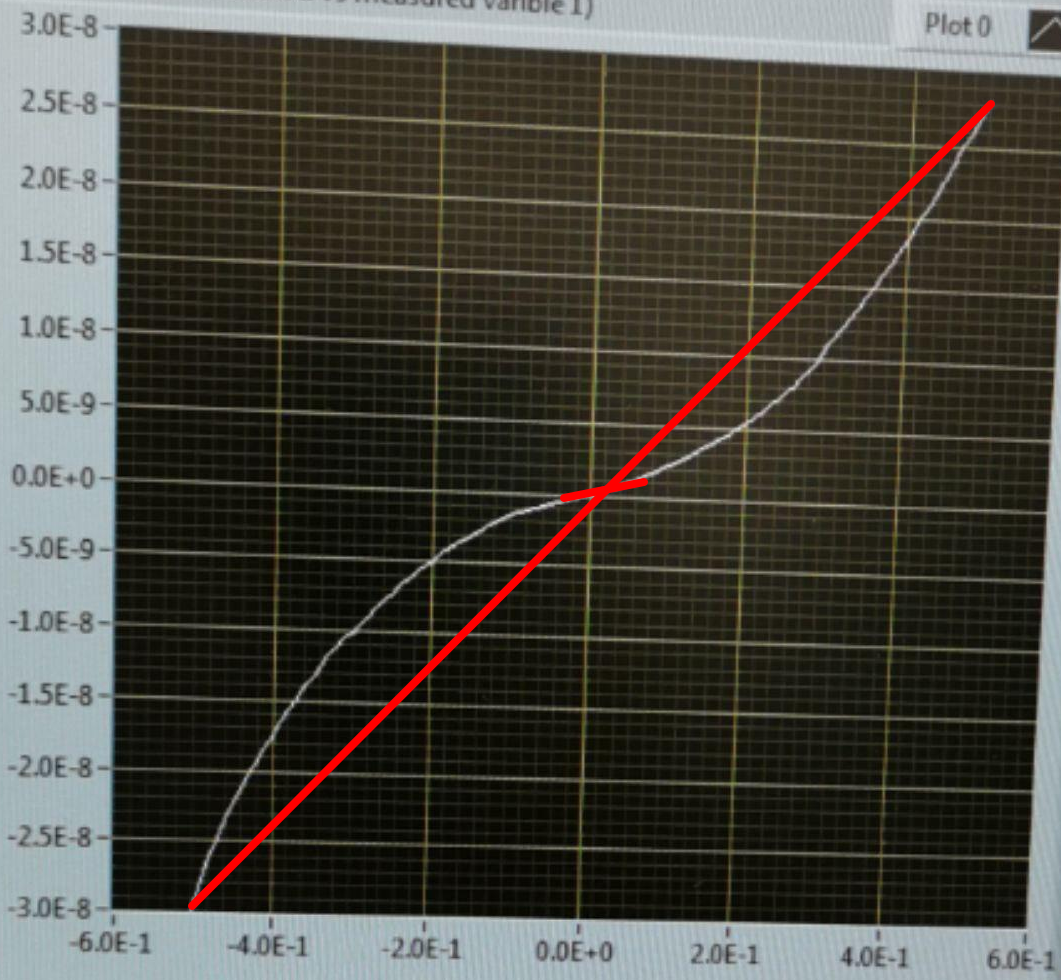
\includegraphics[width=.9\textwidth]{pics/iv_grad.png}
		\end{figure}
	\column{0.49\textwidth}
	\begin{itemize}
		\item G = $\frac{dI}{dV}$ = 4.234E-6
		\item G' = log($|$G$|$) = -5.37
		\item pG = -log($|$G$|$) = 5.37 \me{pondus,power,potential}
%		\item pG = 5.37 \me{$\rightarrow$ 5}
		\item Q: which points best for dV
		\item min max overestimation ? 
		\item average ?
	\end{itemize}
	\end{columns}
\end{frame}

\begin{frame}
	\frametitle[center]{Statistics}
		\begin{figure}
			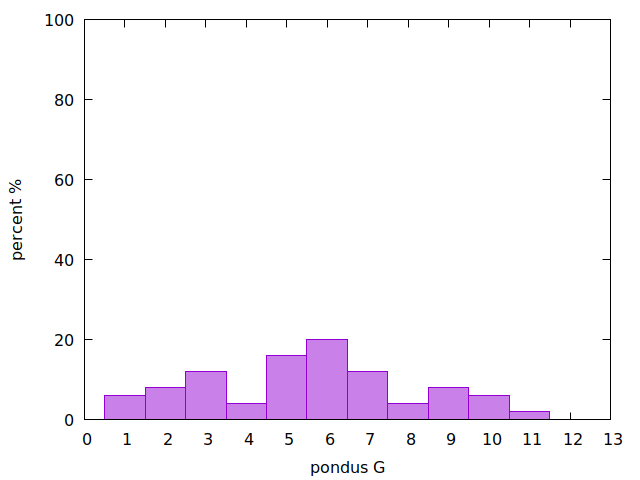
\includegraphics[width=.8\textwidth]{../../Data/I-V/I-V_158_2021_02_26/stat.png}
		\end{figure}
\end{frame}

\begin{frame}
	\frametitle[center]{Statistics}
		\begin{figure}
			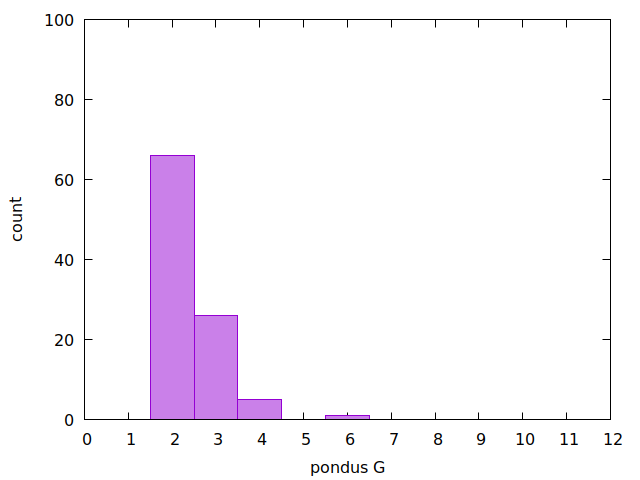
\includegraphics[width=.19\textwidth]{../../Data/I-V/I-V_131_2021_01_20/stat.png}
			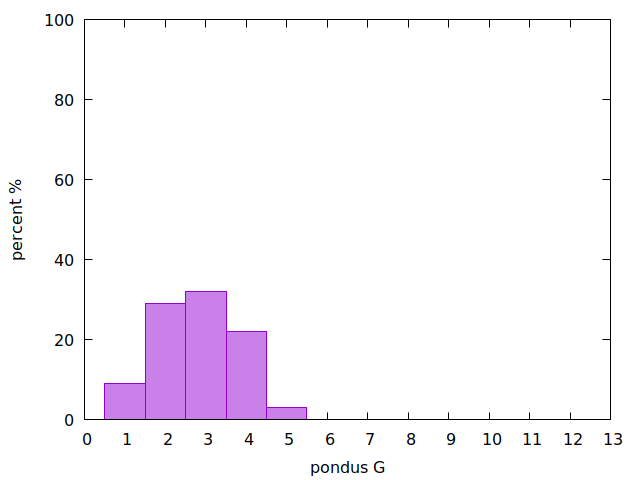
\includegraphics[width=.19\textwidth]{../../Data/I-V/I-V_135_2021_01_20/stat.png}
			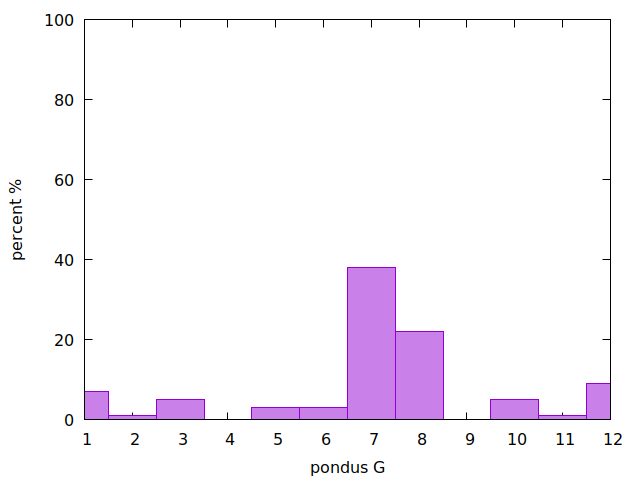
\includegraphics[width=.19\textwidth]{../../Data/I-V/I-V_146_2021-02-23/stat.png}
%			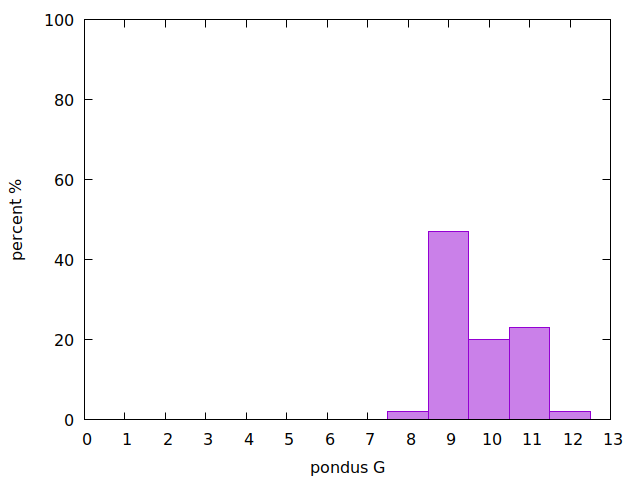
\includegraphics[width=.19\textwidth]{../../Data/I-V/I-V_150_2021_02_03/stat.png}
			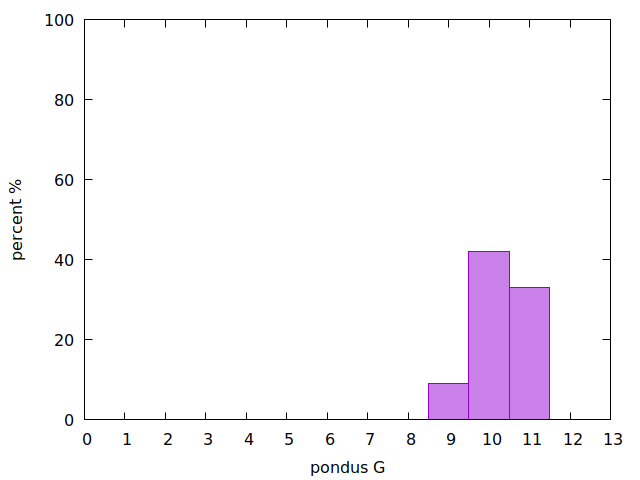
\includegraphics[width=.19\textwidth]{../../Data/I-V/I-V_150_2021_02_09/stat.png}
			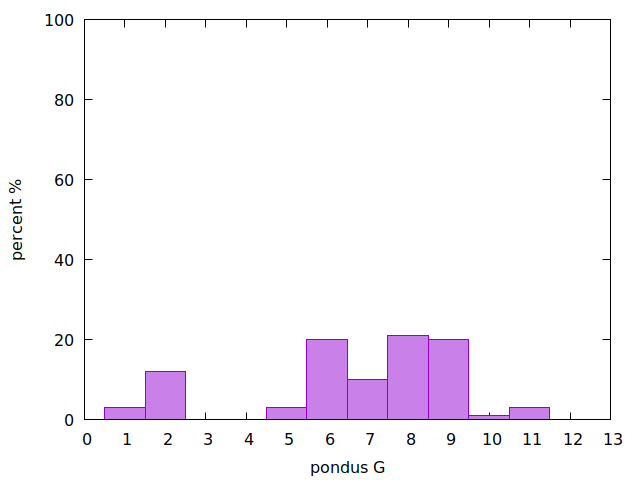
\includegraphics[width=.19\textwidth]{../../Data/I-V/I-V_151_2021_02_05/stat.png}
			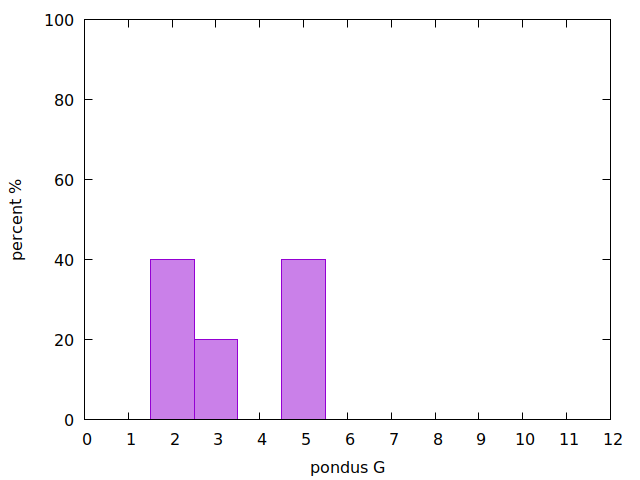
\includegraphics[width=.19\textwidth]{../../Data/I-V/I-V_152_2021_02_09/stat.png}
			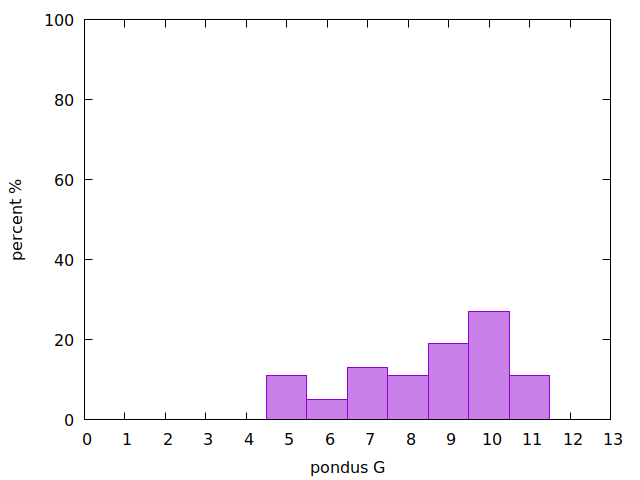
\includegraphics[width=.19\textwidth]{../../Data/I-V/I-V_153_2021_03_03/stat.png}
			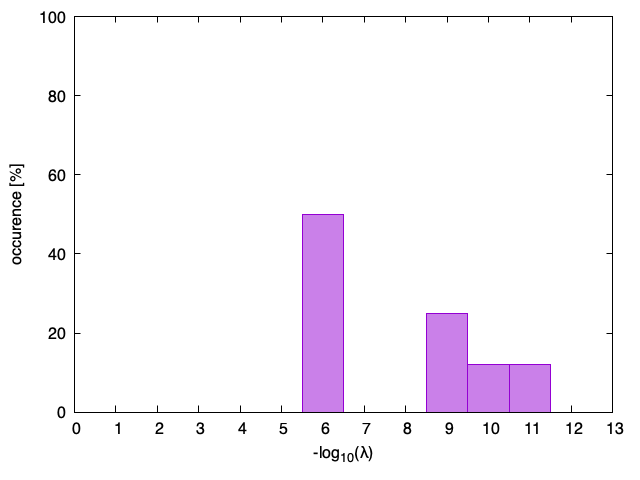
\includegraphics[width=.19\textwidth]{../../Data/I-V/I-V_154_2021_02_23/stat.png}
			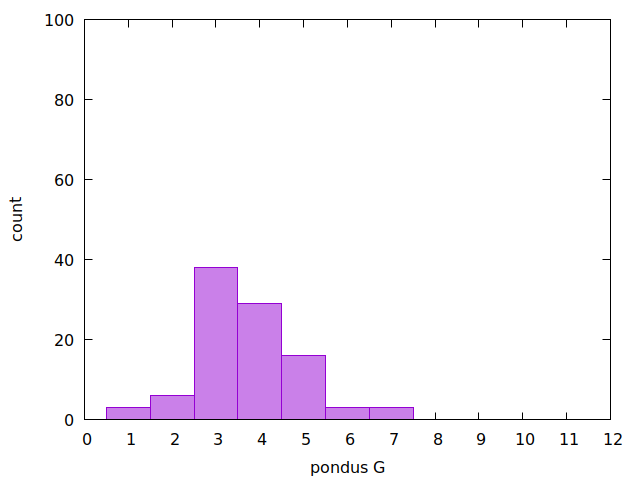
\includegraphics[width=.19\textwidth]{../../Data/I-V/I-V_156_2021_02_23/stat.png}
			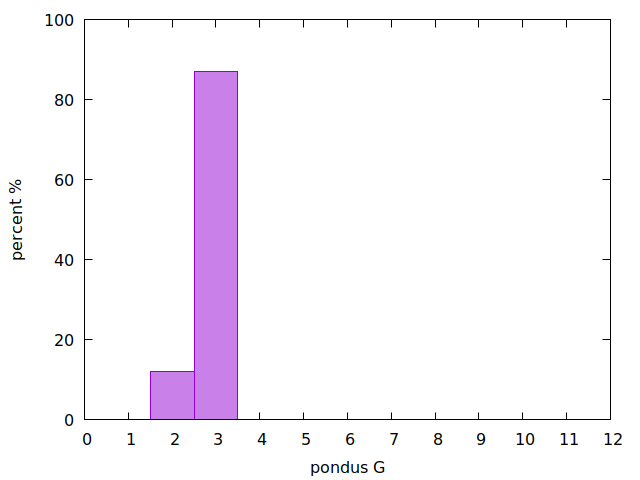
\includegraphics[width=.19\textwidth]{../../Data/I-V/I-V_157_2021_02_25/stat.png}
			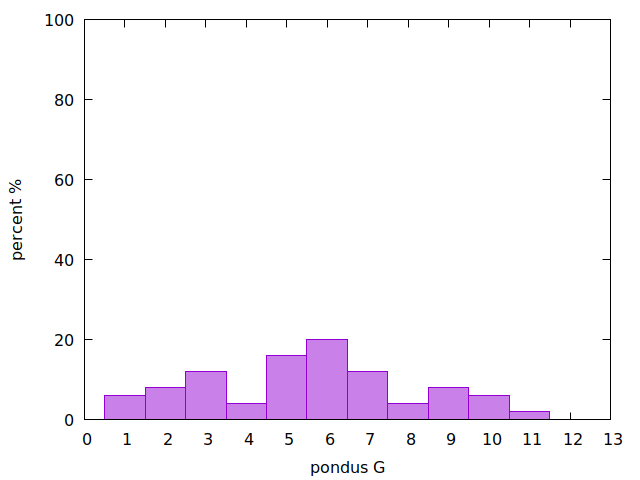
\includegraphics[width=.19\textwidth]{../../Data/I-V/I-V_158_2021_02_26/stat.png}
			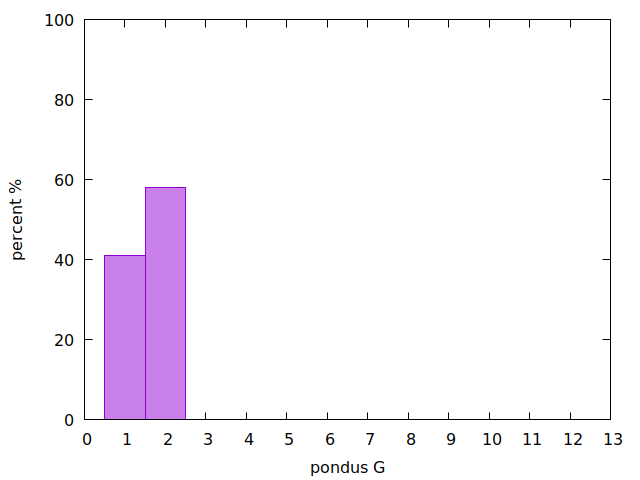
\includegraphics[width=.19\textwidth]{../../Data/I-V/I-V_160_2021_03_01/stat.png}
			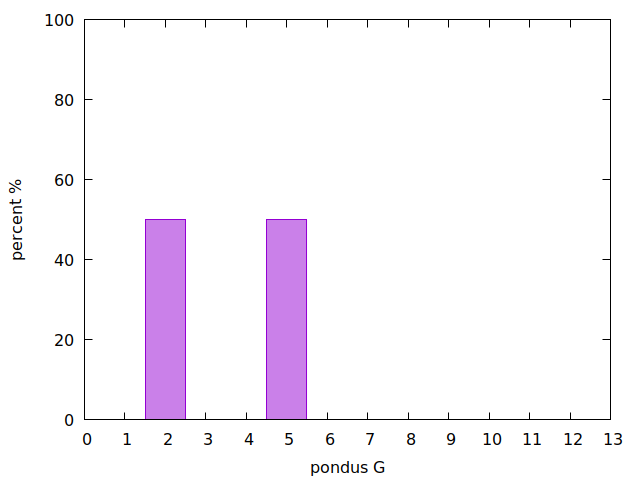
\includegraphics[width=.19\textwidth]{../../Data/I-V/I-V_161_milky_2021_03_01/stat.png}
			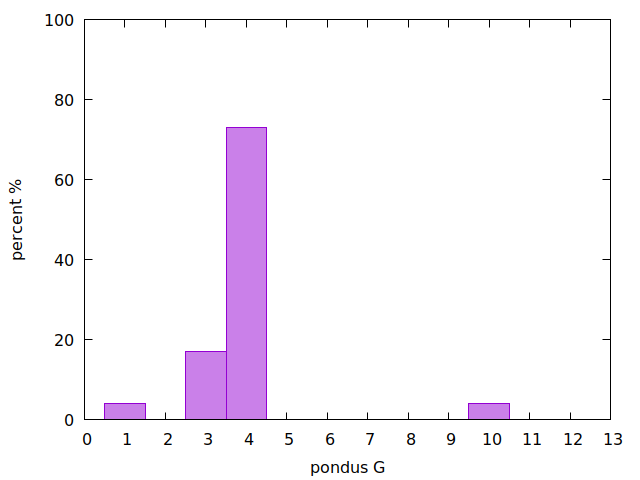
\includegraphics[width=.19\textwidth]{../../Data/I-V/I-V_186_2021_03_01/stat.png}
			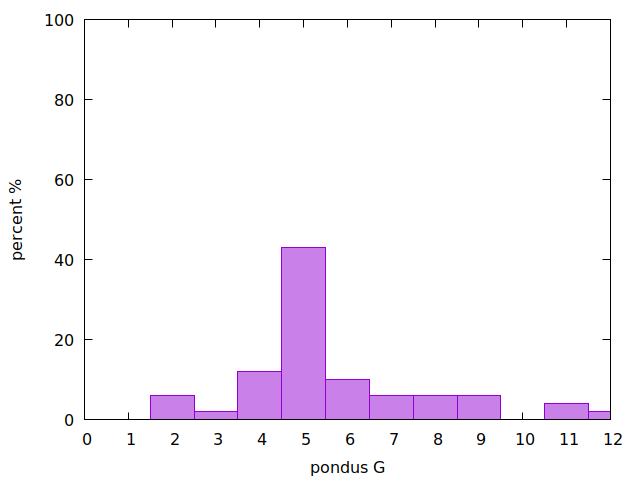
\includegraphics[width=.19\textwidth]{../../Data/I-V/I-V_187_2021_03_03/stat.png}
			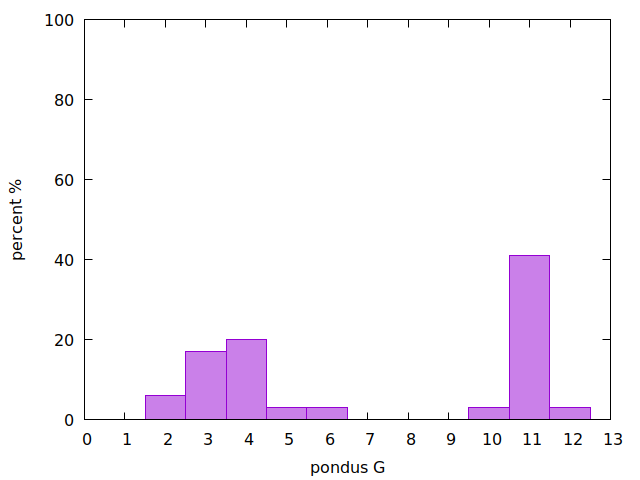
\includegraphics[width=.19\textwidth]{../../Data/I-V/I-V_188_2021_03_03/stat.png}
			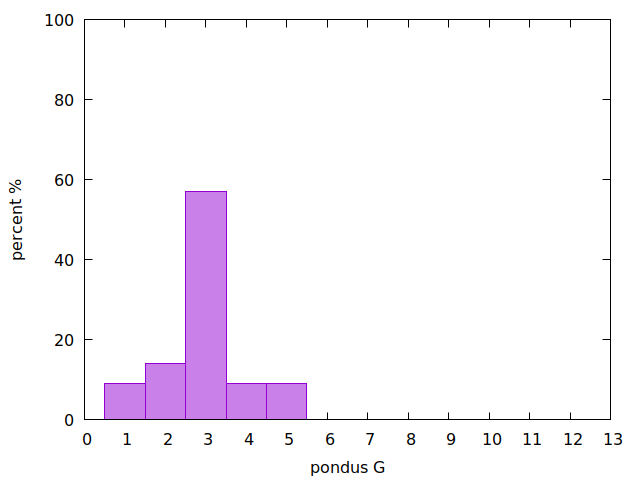
\includegraphics[width=.19\textwidth]{../../Data/I-V/I-V_190_2021_03_04/stat.png}
			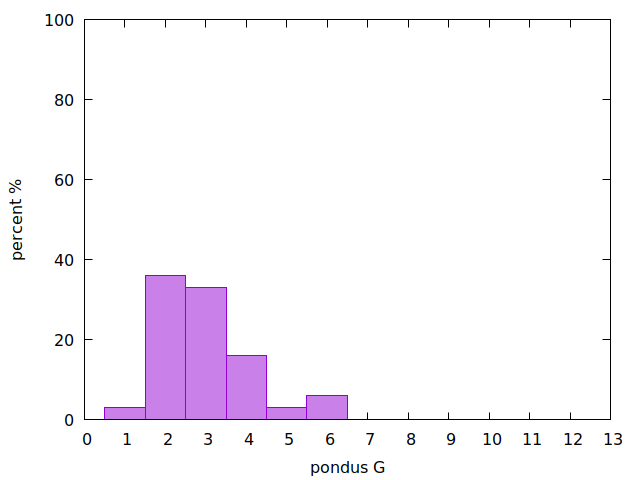
\includegraphics[width=.19\textwidth]{../../Data/I-V/I-V_194_2021_03_04/stat.png}
			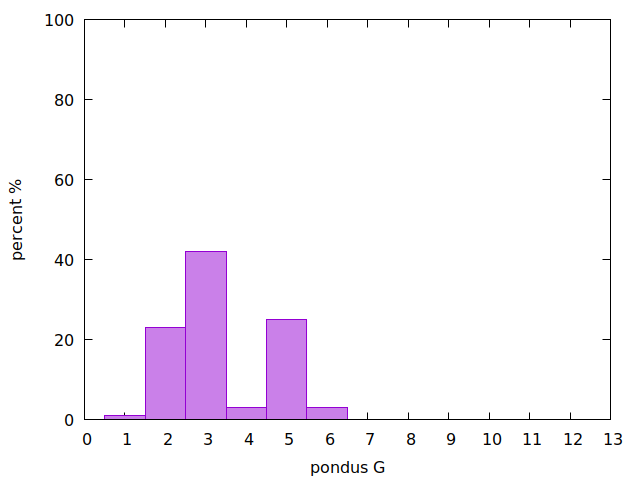
\includegraphics[width=.19\textwidth]{../../Data/I-V/I-V_195_2021_03_04/stat.png}
			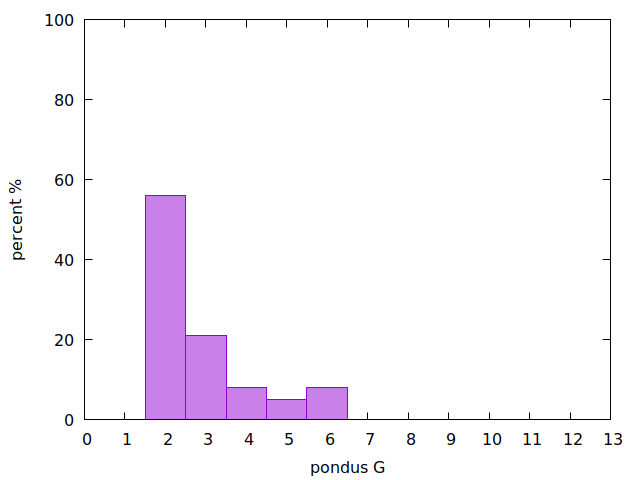
\includegraphics[width=.19\textwidth]{../../Data/I-V/I-V_198_2021_03_04/stat.png}
		\end{figure}
\end{frame}

\begin{frame}
	\frametitle[center]{Best of}
		\begin{figure}
			\begin{subfigure}{.32\textwidth}
				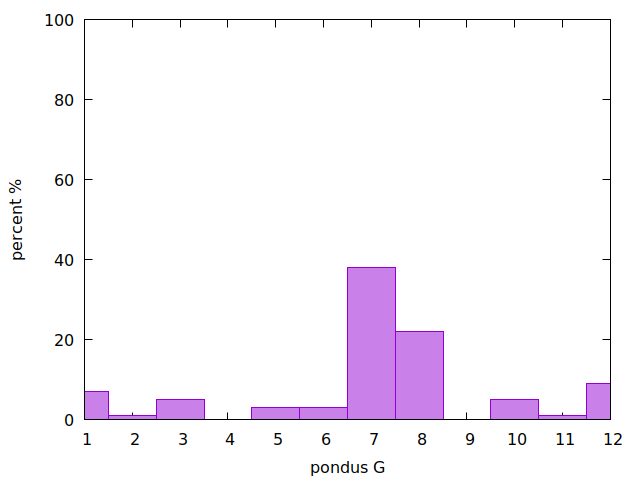
\includegraphics[width=.99\textwidth]{../../Data/I-V/I-V_146_2021-02-23/stat.png}
				\caption{146, 10x1F HG}
			\end{subfigure}
			\begin{subfigure}{.32\textwidth}
				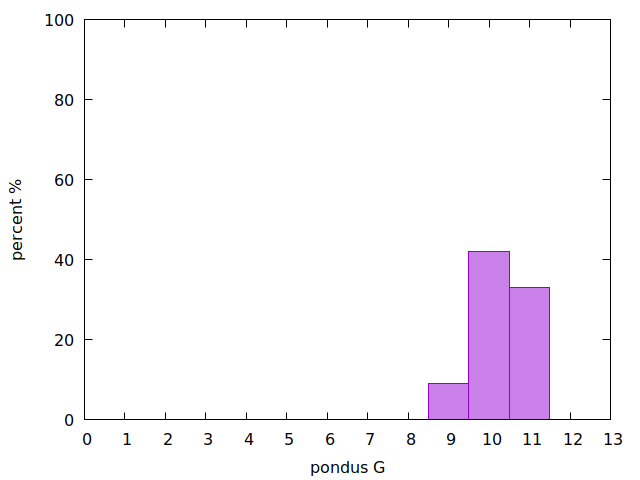
\includegraphics[width=.99\textwidth]{../../Data/I-V/I-V_150_2021_02_09/stat.png}
				\caption{150, 5x2F HG}
			\end{subfigure}
			\begin{subfigure}{.32\textwidth}
				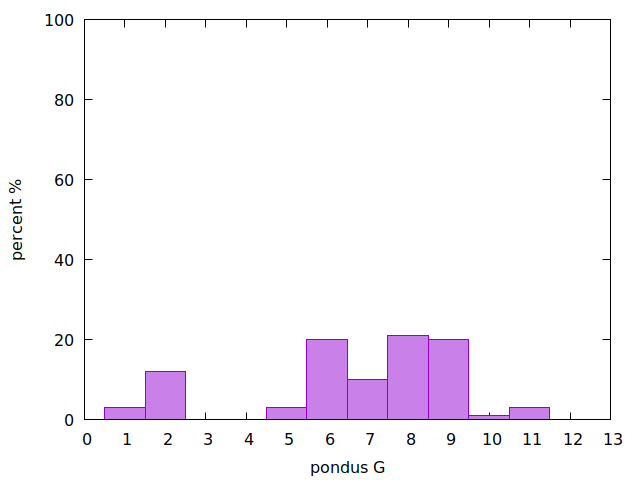
\includegraphics[width=.99\textwidth]{../../Data/I-V/I-V_151_2021_02_05/stat.png}
				\caption{151, 2x2F HG}
			\end{subfigure}
			\begin{subfigure}{.32\textwidth}
				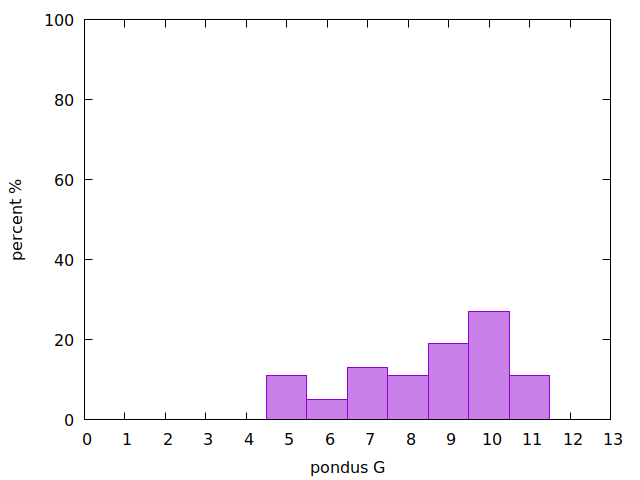
\includegraphics[width=.99\textwidth]{../../Data/I-V/I-V_153_2021_03_03/stat.png}
				\caption{153, 3x4F HG}
			\end{subfigure}
			\begin{subfigure}{.32\textwidth}
				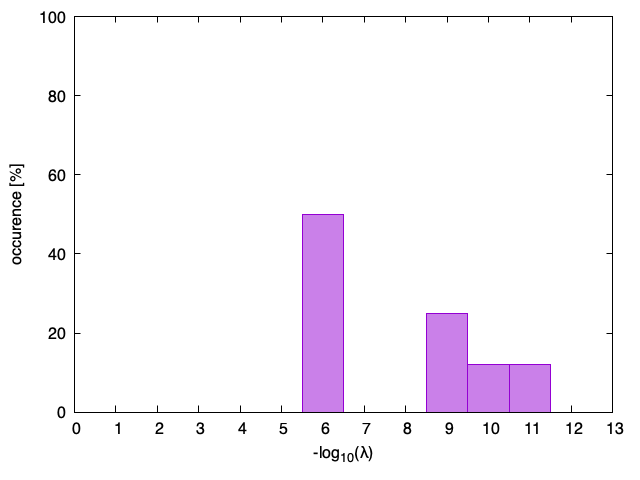
\includegraphics[width=.99\textwidth]{../../Data/I-V/I-V_154_2021_02_23/stat.png}
				\caption{154, 3x4F HG}
			\end{subfigure}
			\begin{subfigure}{.32\textwidth}
				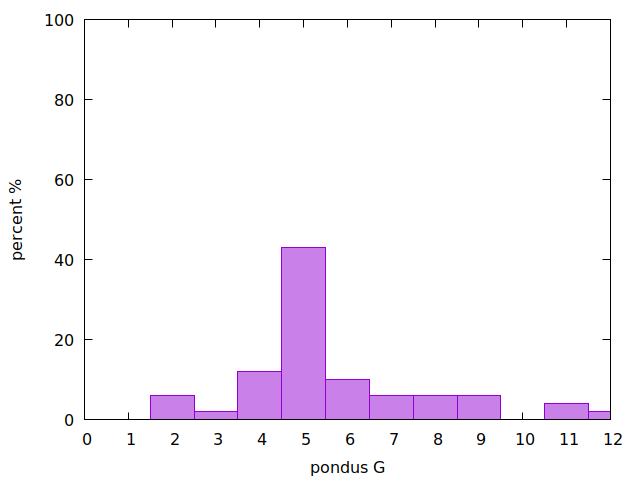
\includegraphics[width=.99\textwidth]{../../Data/I-V/I-V_187_2021_03_03/stat.png}
				\caption{187, 10x1F 5mm/s }
			\end{subfigure}
		\end{figure}
\end{frame}

\begin{frame}
	\frametitle{Optimazation parameters}
	\begin{itemize}
		\item min (average of G )
		\item min (number of hole)
		\item min (layers)
		\item \me{min (calcination temperature)?}
		\item \me{max (DB velocity)?}
		\item \me{max (heating rate)?}
	\end{itemize}
\end{frame}

\begin{frame}
	\frametitle{Optimization meta}
	\begin{itemize}
		\item starting population 10 s
		\item extra entities/experiments per timestep =5 e
		\item 5 time steps 
		\item 1*10+(5-1)*5 = 10+4*5 = 10+20 = 30
		\item 20-30 extra samples for comparison
		\item approx 2-3 hours per sample
	\end{itemize}
\end{frame}


\begin{frame}
	\frametitle{All questions}
	\begin{itemize}
		\item where should be threshold be for holes?
		\item how to calculate derivative?
		\item boundaries for Tcal = [300:500] \me{[400:500]} $^o$C
		\item layers  = [6:14] \me{[4:10]} 
		\item conc = [2:5] \me{[1:5]}
		\item vDoc = [10:20] mm/s
		\item TDOC = [40:80] $^o$C
		\item vCal = [2:16] $^o$C/min
		\item extra steel foil
	\end{itemize}
\end{frame}


%%%%%%%%%%%%%%%%%%%%%%%%%%%%%%%%%%%%%%%%%%%%%%%%%%%%%%%%%%60
\iffalse
\appendix
\begin{frame}
	\frametitle{Frequency Dependence of Permitivity}
\end{frame}
\fi

\end{document}
